\documentclass[12pt, a4paper]{report}
\usepackage[pdftex]{graphicx} %for embedding images
\graphicspath{ {./img/} } %the path to the images
\usepackage[,italian, english]{babel}
\usepackage{url} %for proper url entries,
\usepackage{hyperref}
% \usepackage[bookmarks, colorlinks=false, pdfborder={0 0 0}, pdftitle={<pdf title here>}, pdfauthor={<author's name here>}, pdfsubject={<subject here>}, pdfkeywords={<keywords here>}]{hyperref} %for creating links in the pdf version and other additional pdf attributes, no effect on the printed document
%\usepackage[final]{pdfpages} %for embedding another pdf, remove if not required

\begin{document}
\renewcommand\bibname{References} %Renames "Bibliography" to "References" on ref page


\begin{titlepage}

\begin{center}

\Large \textbf {Programmazione Concorrente e Distribuita - Assigment 03}\\%\\[0.5in]
\vspace{1em}%
\vfill
Leonardo Randacio


Filippo Gurioli


Andrea Biagini
\vspace{1em}
\vfill
{\bf Università di Bologna \\ Scienze e Ingegneria Informatiche}\\[0.5in]

       
\vfill
\today

\end{center}

\end{titlepage}


\tableofcontents
\listoffigures

\newpage
\pagenumbering{arabic} %reset numbering to normal for the main content

\chapter{Analysis}
The goal is to create a Cooperative Sudoku exploiting the \href{https://croquet.io/}{Croquet.io Framework}.

The game is a cooperative version of the classic Sudoku game. The game can be played by any number of players, each player can see the
 board and the numbers placed by the other players. The game is won when the board is completed.

Each player can also be able to see the other players' cursors, and have the capability to exit and join different games at any time.

\section{Task Decomposition}
The game can be decomposed in the following tasks:
\begin{itemize}
    \item \textbf{create game}: create a new game
    \item \textbf{join game}: join an existing game
    \item \textbf{exit game}: exit the current game
    \item \textbf{place number}: place a number in the board
    \item \textbf{move cursor}: move the cursor in the board
\end{itemize}
Each task can be executed by any player at any time.

\section{Data Decomposition}
The game is composed by a board, a set of players, a set of cursors and a set of numbers placed in the board.

\section{Dependency Analysis}
There are two dependency levels.

The first and most visible one is between tasks 
 that belong to different parts of the game. That is the dependency between the place 
 number and move tasks and the create/join/exit task.
 
The second level of dependency is between all tasks that belong to the same part of the game. For example, the place 
 number task is dependent on the move cursor task; the join exit and task is dependent on the create task.

\chapter{Design}
Exploiting \href{https://croquet.io/}{Croquet.io Framework}, the game is designed as a set of objects that communicate with each other via messages.

\section{Croquet.io Framework}
Each object can perform every task of the game and the execution of a task is fired by a message sent to the object.

In order to have all the object be in synch with a coherent game state, Croquet.io provides a shared state that is updated by the objects.
 The shared state is a javascript class that is ensured to be the same on all objects. That is, when an object updates the shared state,
 the change is propagated to all the other objects.

\section{Architecture}
Since the game should provide both the capabilities to create and join games and to play the game,
 the architecture is divided in two macroparts: the lobby and the game. 
 
The lobby is the part of the game where the player can create or join a game.

The game is the part of the game where the player can play the game (and exit). Each user is represented by an object as defined earlier.

\begin{figure}
    \centering
    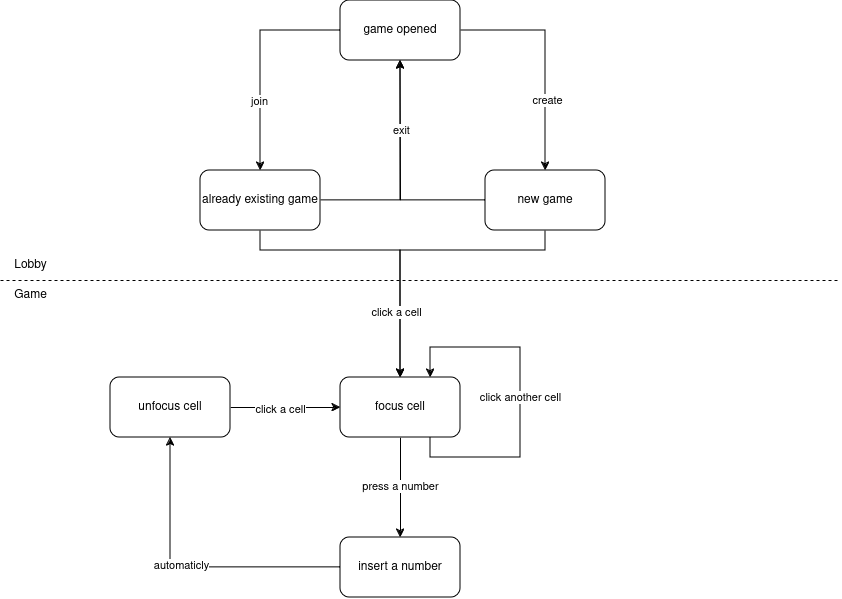
\includegraphics[scale=0.5]{part2a-states.png}
    \caption{UML diagram listing all possible states of the game and how they are related.}
\end{figure}

\begin{figure}
    \centering
    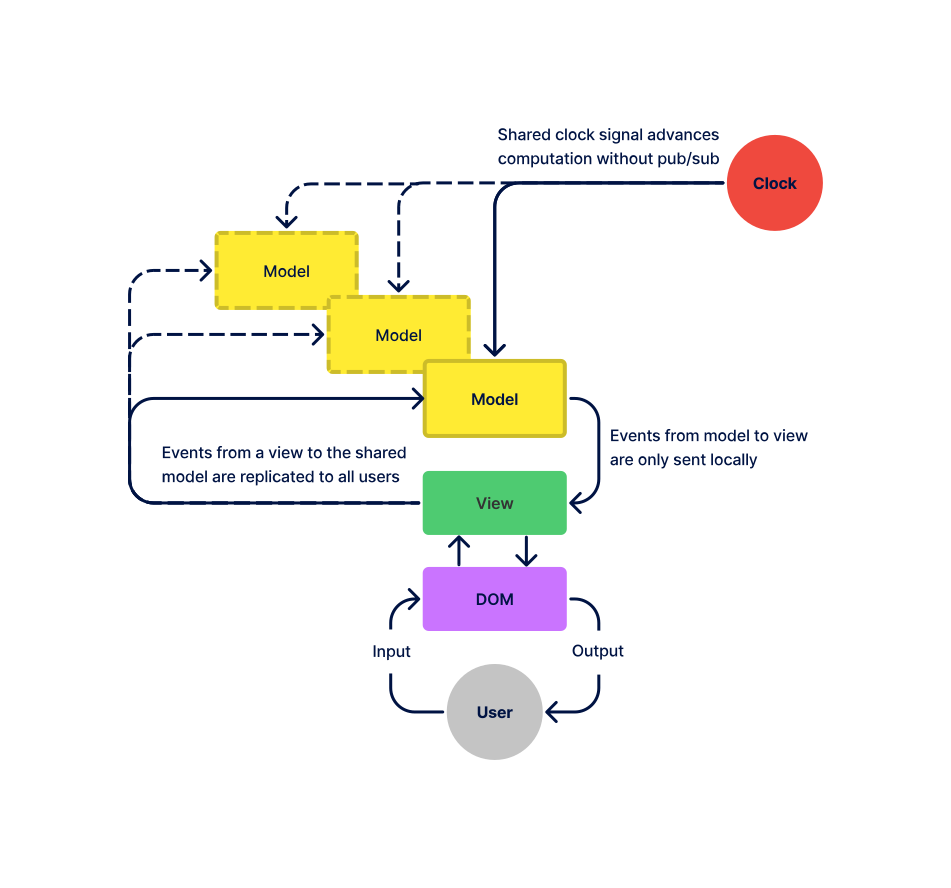
\includegraphics[scale=0.5]{croquet_overview.png}
    \caption{Overview of the croquet.io framework}
\end{figure}

\section{Sudoku Board Generation Inconsistencies}
During the development of the game, an issue was encountered concerning the generation of the Sudoku board. Initially, an online API was used to generate a Sudoku board each time it was queried. Since this operation involves data handling rather than user interface interactions, it was intuitively placed in the shared state, known as the `Model'. The `Model' is replicated across all clients, and executing the board generation operation on all clients led to each client generating a different Sudoku board. This inconsistency occurred because the API call was being made independently on each client's Model, resulting in different boards being generated simultaneously.\\
\\
To solve this issue, the API call has been executed only by the View of the client that is currently creating the new game. In this new version only one client makes the API call to generate the Sudoku board. Once the board is generated, this client updates the shared state with the generated board, ensuring that all other clients receive the same board. By centralizing the API call to a single client and then propagating the result through the shared state, consistency has been obtained across all clients.

\chapter{Implementation}
The project can be divided in two different parts: the first that separates the lobby and the game (as described previously), and the second that separates the model from the view. The model and view are basic Croquet classes used to store data and render the data, respectively. The model is shared among all the clients, while the view is particular to each client. These classes provide basic functionalities but have been extended to ease development further. The extended classes are \texttt{BaseModel} and \texttt{BaseView}. Additionally, we created the \texttt{FirstView} class to fill a gap left by the framework. Croquet.io exposes an update method that is called every frame, but it's guaranteed to be called only for the first view created. The \texttt{FirstView} class is a workaround to ensure the method is fired for every view.\\
\\
The classes that implement the game are \texttt{LobbyModel}, \texttt{LobbyView}, \texttt{GameModel}, and \texttt{GameView}. The model classes are responsible for storing data, while the view classes are responsible for rendering them. Throughout the project, we adhered to a consistent pattern: after a user interaction, a message is sent to the model, which updates the shared state and responds to the view with another message. The view then updates the UI. This pattern is considerably similar to the Remote Procedure Call (RPC) model.

\chapter{Usage}
A bash script \emph{boot.sh} is provided to run the application.

The script uses openssl, so the user should ensure it is installed on the system.

The script generates artifacts for the correct functioning of the program and installs node dependencies.

After running the script once, subsequent runs can be performed by simply executing the \emph{node app} command from cli.

\chapter{Conclusion}
The project was successfully implemented and tested. The game is fully functional and can be played by any 
 number of players, also providing fault tollerance. The cooperative Sudoku project demonstrates the potential and
 flexibility of the Croquet.io framework in developing interactive and collaborative applications. The simple and 
 intuitive API allows for rapid development and easy testing of applications.

\bibliographystyle{plain}
\bibliography{References}

\end{document}